\section{Logics}
This section describes the ''machinery'' behind the simulations. How the system (i.e. bulk or surface) is represented and how simulations are performed will be detailed from a computer science point of view.
\subsection{The Atoms}
The system contains a number of individual atoms. Each atom is stored
as a separate instance of an atom class, containing, among other things, the
atom's mass, current velocity, position and acceleration.
\subsection{The Verlet List}
When the simluations are run, an array of Verlet Lists (one for each atom in the system) is created, where each entry is a linked list containing all the atoms inside the Verlet skin of the current atom. That is, Verlet list ''i'' contains atom ''i'' and all of its' neighbors. The Verlet lists are updated by looping through all the atoms in the system and adding all atoms that are within the Verlet skin. To avoid double counting of the forces, only one of the atoms who are in each other's Verlet skin are added to the other. That is, if atoms ''i'' and ''j'' are within each other's Verlet skin, only atom ''j'' is added to the Verlet skin of atom ''i'' and not vice versa.

\begin{figure}
\centering
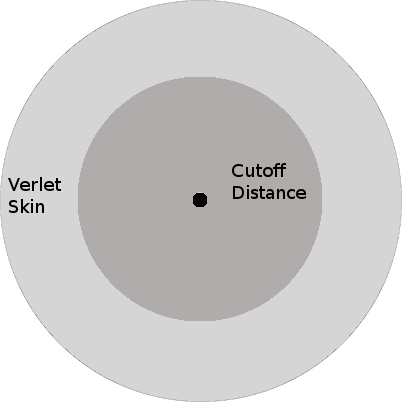
\includegraphics[width=7cm]{Verlet_list.png}
\caption{Verlet skin and cutoff distance for an atom}
\label{fig:verlet_list}
\end{figure}
\subsubsection{Updating the Verlet Lists}
The update of the Verlet lists is a huge time sink and also has a time complexity $\Theta(N^2)$, which gives a rapid increase of the time consumption for increasing number of atoms. It is thus important to avoid any unnecessary updates. The Verlet lists are only updated when the total displacement of the two atoms that have moved the most in the system, is greater than the difference between the Verlet skin and the cutoff distance of the force calculations.
That update occurs if and only if
\[
\max_{i=1,\ldots,N}(\texttt{disp}_i) + \max_{i \neq j}(\texttt{disp}_j) \geq
\texttt{Verlet Skin} - \texttt{cutoff}
\]
Thus the Verlet lists are updated only when it is probably needed. It is, however, still updated a bit more often than absolutely necessary.

\subsection{The Verlet Integrator}
For the integration of the equations of motion for each atom, a numerical integrator is required. In this program the Velocity Verlet algorithm is used, since it offers a good balance between complexity and stability, i.e. time to perform calculations versus accuracy of calculations. The integration is performed in two steps. First the new position of each atom is calculated depending on the current velocity and accceleration of the atom. In the second step the new velocity and new acceleration of each atom is calculated based on the new position and the current as well as the future accelerations.

Below is the Velocity Verlet algorithm
\begin{equation}
\bar{x}(t + \Delta t) = \bar{x}(t) + \bar{v}(t)\Delta t +
\frac{1}{2}\bar{a}(t)\Delta t^2
\end{equation}
\begin{equation}
\bar{v}(t + \Delta t) = \bar{v}(t) + \frac{\bar{a}(t) + \bar{a}(t+\Delta t)}{2}\Delta t
\end{equation}

\subsubsection{Force Calculation}
According to Newton's second law $\bar{F} = m*\bar{a}$, the net force acting on
each atom is required in order to calculate the acceleration.

The Lennard-Jones potential is used in this program:
\begin{equation}
V_{LJ} = 4\epsilon\left( \left(\frac{\sigma}{r}\right)^{12} - \left(
\frac{\sigma}{r} \right)^6 \right)
\end{equation}
Where $\epsilon$ and $\sigma$ are material parameters.
And using the fact that 
\begin{equation}
\bar{F} = -\nabla(V)
\end{equation}
the force acting on each atom can be calculated only using the current position.
In order to save computations Newton's third law is utlized: $\bar{F}_{ij} = -
\bar{F}_{ji}$

Since a truncated Lennard-Jones potential is used, only the force between atoms that are witihng the cutoff distance of each other is calculated. Thus when the force is calculated, only the atoms that are in the Verlet list of the current atom, and are within the cutoff distance, are considered.
